\section*{Exercises}

\hrulefill

\textbf{Ex.} In parsing, ...
\begin{compactitem}[$\quad\bullet$]
	\item[$\square$] LL(1) parsers are more powerful than LR(0) parsers.
	\item[$\boxtimes$] LR(1) parsers are more powerful than LL(1) parsers.
	\item[$\boxtimes$] LALR(1) may introduce new reduce/reduce conflicts compared to LR(1) when parsing the same grammar.
	\item[$\square$] LALR(1) may introduce new shift/reduce conflicts compared to LR(1) when parsing the same grammar.
\end{compactitem}

\hrulefill

\textbf{Ex.} For context free grammars, ...
\begin{compactitem}[$\quad\bullet$]
	\item[$\boxtimes$] LR parsers can handle left-recursive grammars.
	\item[$\boxtimes$] LR parsers can handle right-recursive grammars.
	\item[$\square$] LL parsers can handle left-recursive grammars.
	\item[$\square$] LR(0) parsers are more powerful than LL(1) parsers.
	\item[$\boxtimes$] even with an unambiguous CFG, there may be more than one derivation.
\end{compactitem}

\hrulefill

\textbf{Ex.} A left-recursive grammar cannot be implemented by an LL(k) parser for any k.
$$ \boxtimes \text{ True } \qquad \square \text{ False }$$

\hrulefill

\textbf{Ex.} LR(k) grammars cannot be right recursive.
$$ \square \text{ True } \qquad \boxtimes \text{ False }$$


\hrulefill

\textbf{Ex.} There is no such thing as a shift/shift conflict for a LR parser.
$$ \boxtimes \text{ True } \qquad \square \text{ False }$$


\hrulefill

\textbf{Ex.} Calling conventions, ...
\begin{compactitem}[$\quad\bullet$]
	\item[$\boxtimes$] specify where arguments and return values should be stored.
	\item[$\square$] specify the starting address of stack and heap.
	\item[$\boxtimes$] can be disregarded by the compiler for functions that are not exposed to external callers as an optimization.
\end{compactitem}

\hrulefill

\textbf{Ex.} Any type-safe program, ...
\begin{compactitem}
	\item[$\boxtimes$] can raise en exception.
	\item[$\square$] can treat non-code values as code.
	\item[$\square$] always terminates.
	\item[$\boxtimes$] can raise a segfault (unsure).
\end{compactitem}

\hrulefill

\textbf{Ex.} Nominal subtyping, ...
\begin{compactitem}[$\quad\bullet$]
	\item[$\boxtimes$] requires us to explicitly declare subtyping relationships.
	\item[$\square$] is used by OAT for struct subtyping.
	\item[$\square$] is a subcategory of structural subtyping.
	\item[$\boxtimes$] is used by Java for subtyping.
\end{compactitem}

\hrulefill

\textbf{Ex.} A basic block, ...
\begin{compactitem}[$\quad\bullet$]
	\item[$\boxtimes$] starts with a label.
	\item[$\square$] can contain more than one control-flow instruction.
	\item[$\boxtimes$] is always executed starting from the basic block's first instruction.
\end{compactitem}

\hrulefill

\textbf{Ex.} Strength reduction, ...
\begin{compactitem}
	\item[$\square$] refers to a class of optimizations that can be profitably applied irrespective of the target architecture.
	\item[$\boxtimes$] is applicable to loops, by creating a dependent induction variable.
	\item[$\square$] can only be meaningfully applied if the IR on which the optimization is applied is in SSA form.
	\item[$\square$] reduces the static number of operations that are performed.
\end{compactitem}

\hrulefill

\textbf{Ex.} Which of the following are examples of forward analysis?
\begin{compactitem}
	\item[$\square$] Liveness analysis
	\item[$\boxtimes$] Available expressions
	\item[$\boxtimes$] Available registers
\end{compactitem}

\hrulefill

\textbf{Ex.} Which of the following statements are true?
\begin{compactitem}
	\item[$\square$] Contradictory to its name, the linear scan register allocation runs in a log-linear time in the number of program variables.
	\item[$\square$] Spilling two registers is always less efficient than spilling one.
	\item[$\square$] To apply linear scan register allocation, we need to compute the reaching definitions and the liveness analysis.
\end{compactitem}

\hrulefill

\textbf{Ex.} Consider the following dominance frontier DF of a graph:
DF[$ U $] = $\{ Y \}$,
DF[$ V $] = $\{ Z, W, Y \}$,
DF[$ W $] = $\{ V, Y \}$,
DF[$ X $] = $\{  \}$,
DF[$ Y $] = $\{ V \}$,
DF[$ Z $] = $\{  \}$.
There is a variable $x$ that is modified at nodes $N = \{X, Y, Z\}$. Determine all nodes
where $\phi$ functions for $x$ have to be inserted, i.e., the join points for $N$ with respect to $x$.
Determine the least fixed point of the sequence:
$$J[N] = \text{DF}_k[N] \text{ where } \text{DF}_0[N] = \text{DF}[N]; \text{DF}_{i+1}[N] = \text{DF}[\text{DF}_i[N] \cup \{N\}]$$\smallskip

$\text{DF}_0[\{X, Y, Z\}] = \{V\}$,

$\text{DF}_1[\{X, Y, Z, V\}] = \{V, W, Z, Y\}$,

$\text{DF}_1[\{V, W, Z, Y\}] = \{V, W, Z, Y\} = J[\{X, Y, Z\}]$

\hrulefill

\textbf{Ex.} What are the types of the followint \texttt{getelementptr} instructions?
\begin{lstlisting}
	struct B {
		int64_t c;
		struct B *d;
		struct A e[10][10];
	}; 
\end{lstlisting}

\texttt{getelementptr \%struct.B* @g, i64 0} : \textcolor{blue}{\texttt{struct.B*}}

\texttt{getelementptr \%struct.B* @g, i64 0, i64 0} : \textcolor{blue}{\texttt{i64*}}

\texttt{gep \%struct.B* @g, i64 0, i64 2, i64 5} : \textcolor{blue}{\texttt{[10 x struct.A]*}}

\hrulefill

\textbf{Ex.} If we try to precolor nodes in an inference graph while adhering to the calling convention, what problem might we face?\medskip

The problem is that multiple return values and arguments that interfere with each other must use the same registers.

\hrulefill

\textbf{Ex.} Apply Mark and Sweep:

\vspace{-11pt}
\begin{center}
	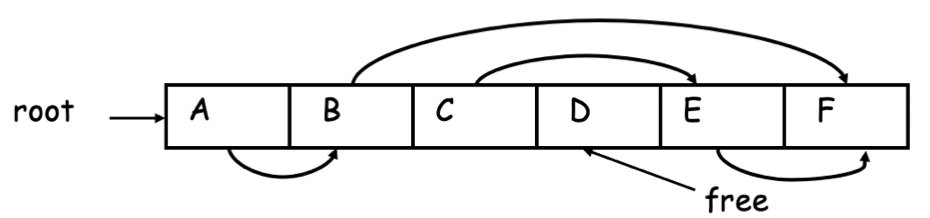
\includegraphics[width=0.5\linewidth]{before_ms.png}
\end{center}

\begin{multicols*}{2}
	After Mark:

	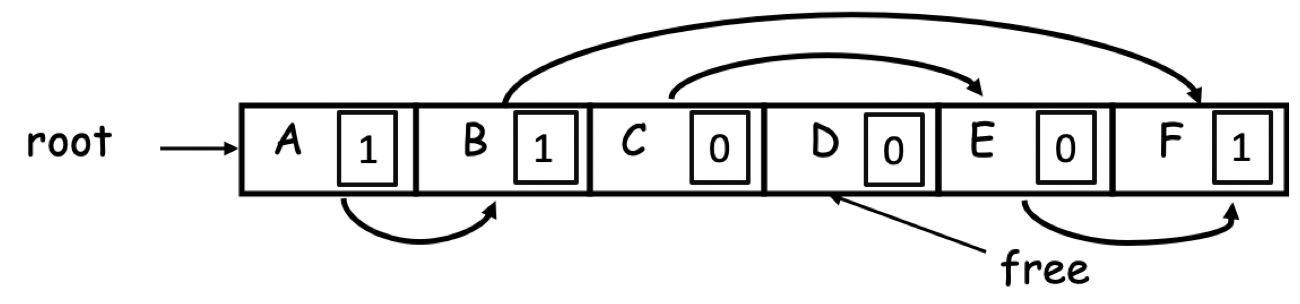
\includegraphics[width=\linewidth]{mark.png}

	After Sweep:

	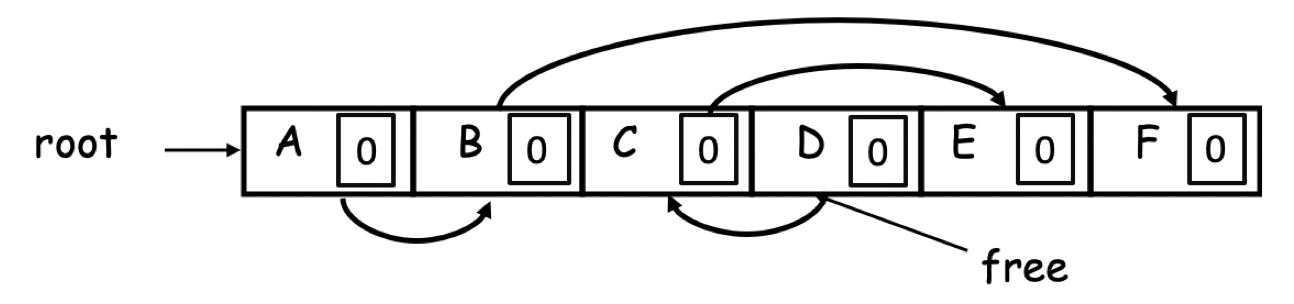
\includegraphics[width=\linewidth]{sweep.png}
\end{multicols*}

\hrulefill

\textbf{Ex.} Apply Stop and Copy:
\begin{multicols*}{2}
	Before:

	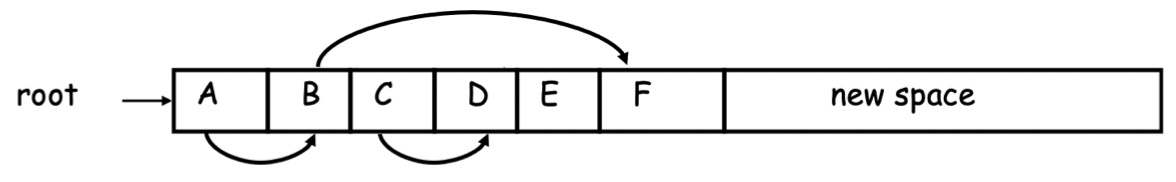
\includegraphics[width=\linewidth]{before_sc.png}
	\columnbreak

	After:
	\vspace{-11pt}

	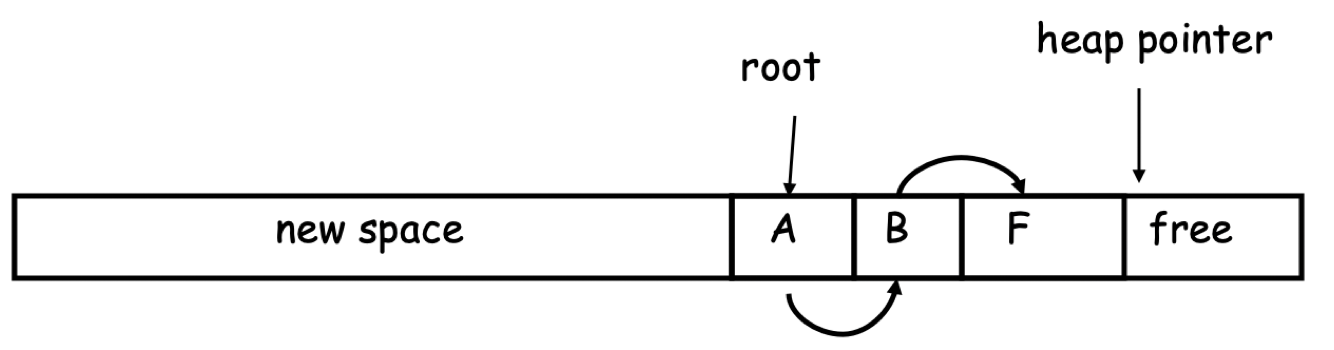
\includegraphics[width=\linewidth]{after_sc.png}
\end{multicols*}
